% Une ligne commentaire débute par le caractère « % »

\documentclass[a4paper]{article}

% Options possibles : 10pt, 11pt, 12pt (taille de la fonte)
%                     oneside, twoside (recto simple, recto-verso)
%                     draft, final (stade de développement)

\usepackage[utf8]{inputenc}   % LaTeX, comprends les accents !
\usepackage[T1]{fontenc}      % Police contenant les caractères français
\usepackage[francais]{babel}
\usepackage{fullpage}
\usepackage{multicol}
\usepackage{hyperref}
\hypersetup{
    colorlinks=true,
    linkcolor=blue,
    filecolor=magenta,      
    urlcolor=red
    }
\usepackage{bookmark}
\usepackage{blindtext}
\setlength\columnsep{30pt}



\usepackage{graphicx}  % pour inclure des images
\graphicspath{ {rapport/img/} }

%\pagestyle{headings}        % Pour mettre des entêtes avec les titres
                              % des sections en haut de page

\title{  TP2 : Les capteurs\\Programmation mobile}
\author{Mohamad Satea Almallouhi - Tony Nguyen\\\emph{M1 Génie Logiciel}\\Faculté des Sciences\\Université de Montpellier.}
\date{5 mars 2024}



\begin{document}
    \maketitle
    \begin{center}
        
\includegraphics[height=.95\textwidth]{power}
    \end{center}

    \begin{abstract}     % Résumé du travail
      \emph{Nous avons réalisé une application Android en Java afin de démontrer l'utilisation des capteurs intégré.}
    \end{abstract}
    \newpage
    %\dominitoc  % initializer les minitoc
    \tableofcontents

    \newpage
    \begin{multicols}{2}
        [
            To Do
            \begin{itemize}
                \item diagram use case
                \item diagram sequence for synchronisation
                \item diagram state machine w/ tikz library to describe save function
                \item add code picture
                \item add smartphone picture
                \item ask Satea for part 2 \& 3 explanation
                \item !!! make an .apk file for easy install, no compilation !!!
                \item diagram class observer DONE
                \item diagram class observer specific (Fragment Manager)
            \end{itemize}
        %     Faire une vidéo, le rapport avec des screenshot des résultats et du code et enfin un read.md(instruction). En plus, pour le bonus, faire une belle application, des tests unitaires, utiliser Kotlin, faire le rapport en Latex.
        ]
        \section*{Introduction}
            \addcontentsline{toc}{section}{Introduction}
            \paragraph{}
                Dans le cadre de l'Unité d'Enseignement Programmation Mobile, nous allons voir comment utiliser des fragments et la persistance des données.
            \paragraph{}
                Les sections du rapport suit les exercices.
        \section*{Démonstration vidéo}
            \addcontentsline{toc}{section}{Démonstration}
        \section{Fragment}
            \paragraph{}
                Un fragment est une portion réutilisable de l'interface utilisateur de notre application. Ils sont utiles car ils sont modulaires et réutilisables. 
            \paragraph{}
                Dans cette section, nous allons voir comment les créer, les afficher et comment les faire communiquer entre eux.
            \subsection{Création}
                \paragraph{}
                    Afin de créer un nouveau fragment, il nous suffit d'hériter de la classe de base Android : "\emph{Fragment}".

                    Pour spécifier le comportement du nouveau fragment, il nous suffira de masquer la méthode \textbf{onCreateView()}.

                    Dans ce TP, nous avons créer 2 fragments, \textbf{UserInputFragment} et \textbf{DisplayFragment}.

                    (UserInputFragment, DisplayFragment extends Fragment)
            \subsection{Ajout}
                \paragraph{}
                    Pour pouvoir les afficher, nous avons créer une activity et son layout vide.
                    
                    Nous avons ensuite, ajouté une balise \textbf{fragment} pour chaque fragment crée. Il faut remarquer 2 attributs important.

                    L'attribut \textbf{android:name} associe cette balise .xml à aux classe fragment crée dans la sous-section précédente.

                    L'attribut \textbf{tools:layout} associe cette balise au layout indiqué.

                    Nous savons à présent comment créer un fragment, et l'afficher.
                    
                    tag fragment - attribut name pour la classe et attribut layout pour la vue
                    \\
                    Start\_toStartOf
                    Top\_toTopOf 
                    ...
            
            \subsection{Couper l'écran en 2}
                C'était trop dur.
            \subsection{Communication entre fragment}
                \paragraph{}
                    Avant la communication, il est nécessaire de transmettre notre \emph{ModelView} contenant les différentes MutableLiveData.
                \paragraph{}
                    Une fois le model placé dans le \emph{Bundle}, nous pouvons envoyer le message. Pour faire cela, nous utilisons la méthode \textbf{setFragmentResult(String requestKey, Bundle result)} pour envoyer les données (contenus dans le bundle avec requestKey une chaine de charactères fixés à l'avance par le programmeur, le fragment receveur devra utiliser la même requestKey).
                
                \paragraph{}
                    Le message est maintenant envoyé, nous allons voir comment le recevoir.

                    Il sera nécessaire d'utiliser la méthode \textbf{setFragmentResultListener()} de la classe \emph{FragmentManager}.

                    L'argument listener sera une classe anonyme qui hérite de \emph{FragmentResultListener} dans laquelle on masque la méthode \textbf{onFragmentResult()}. Si nous avons bien utilisé les même requestKey, alors l'argument bundle contiendra les bonnes données. À partir de là, nos fragments possède la même instance du model.
            \subsection{La synchronisation et mise à jour}
                \paragraph{}
                    Lors de la détection d'un changements, nous souhaitons publié le changement et mettre à jour la vue. Pour cela, nous allons accéder aux différents \emph{MutableLiveData} dans notre \emph{ModelView} : \emph{UserInputViewModel}. Une fois fait, nous publions simplement la nouvelle valeur avec la méthode \textbf{postValue()}. Nous envoyons les valeurs lorsque l'utilisateur appuie sur "Submit" ou après qu'il ait selectioné l'option "Synchronise" puis modifie le texte.
                \paragraph{}
                    Afin d'être notifié des plublications, il faut s'abboner aux MutableLiveData et les \textbf{observer}.
                \paragraph{}
                    Receiving
                    \\
                    get the MutableLiveData from ViewModel and observe
                    \\
                    Quand l'observateur est notifié, la méthode \textbf{onChanged()} est appelé et la nouvelle valeur est placé dans une \emph{<TextView>}.
            \subsection{Observer}
                % To Do
                % \begin{itemize}
                %     \item diagram class observer
                %     \item diagram class observer specific (Fragment Manager)
                % \end{itemize}
                \paragraph{}
                    Voici un rappel du diagramme de classe du patron de conception \emph{Observateur} 
                    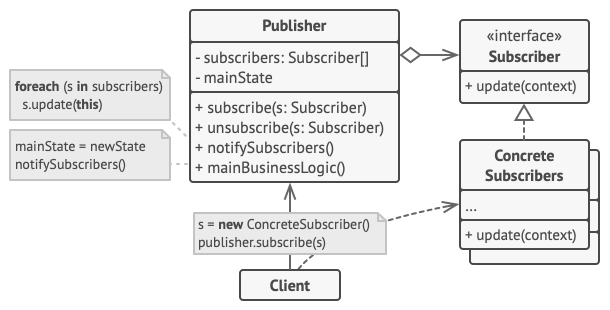
\includegraphics[width=.49\textwidth]{observer}
                \paragraph{}
                    Il faut remarquer que ce design pattern est essentiel dans ce tp pour implémenter la communication entre les fragments. On y retrouve les méthodes de souscriptions, notifications et mises à jour.

                    On identifie les méthodes de notifications comme \textbf{setFragmentResult()} et \textbf{postValue()}.

                    Les méthodes de mises à jour correspondendt à \textbf{setFragmentResultListener()} et \textbf{observe()}.
        \section{Persistance}
            \paragraph{}
                Nous allons maintenant nous intéressé à la sauvegarde sur le long terme.
            \subsection{Sauvegarde}
                Lors d'un clique sur le boutton \emph{"Save"}, une écriture sur le stockage local du smartphone est enclenché.

                La méthode \textbf{saveJsonToFile()} se chargera d'écrire dans le fichier \emph{test.json}. 
            \subsection{Saisie automatique}
        \section{Réseau}
            Cet exerice n'a pas été réalisé.
        \section{Service}
            \paragraph{}
                Après qu'une écriture sur le stockage du téléphone a été faite, il nous est possible de récupérer le contenu de ce fichier et de l'afficher à l'utilisateur.

                À l'appuie du boutton "load", le service est démaré. \emph{FileDownloadService} va simplement lire le fichier de sauvegarde prédéfini \emph{test.json}.

                Il va ensuite, diffuser les valeurs à travers un le \emph{LocalBroadcastManager}.
            \paragraph{}
                Dans le DisplayFragment, Nous nous mettons à l'écoute du broadcast. 

                
                
                À la reception du broadcast, le text est écrasé par les différentes valeurs contenus dans le fichier.


        % \section{Bonus: LifeCycle}
        % \section{Bonus: ViewModel}
        % \section{Bonus: LiveData}
        % \section{Bonus: Room}
    \end{multicols}
\end{document}
Quand on quitte l'appli, onStop et onSaveInstanceState sont invoqués.
Quand on fait retour, onStop est invoqué.
Quand on revient, onStart et onViewCreated sont invoqués.